\shorthandoff{:!} %règle un problème de compatibilité avec babel
%
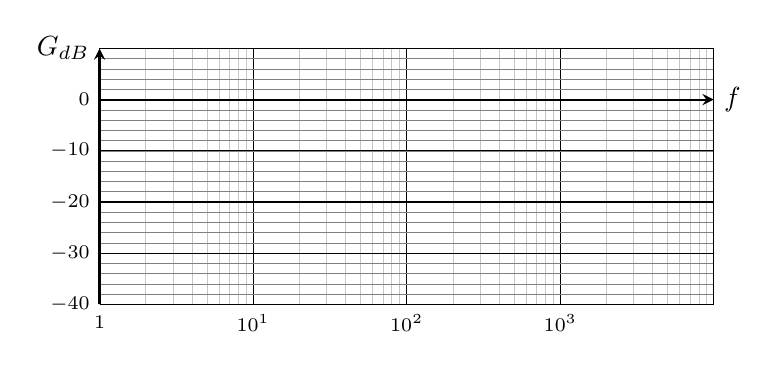
\begin{tikzpicture}[scale=0.65,rotate=0]
	% Dimensions du repere
	\def\xlrg{12} \def\ylrg{5}
%
% Tracé de l'axe log base 10
	\foreach \ee in{0,1,2,3}{
		\foreach \x in {1,2,...,10} {
			\draw[very thin,color=gray!45] ({\xlrg/4*ln(\x*10^\ee)/ln(10)-\xlrg},0)--({\xlrg/4*ln(\x*10^\ee)/ln(10)-\xlrg},-\ylrg);
		};
	};
%tracé de la légende pour les puissances de 10
	\foreach \ee in{1,2,3}{
	\foreach \x in {10}
	{\draw[thin,color=black]({\xlrg/4*ln(\x^\ee)/ln(10)-\xlrg},0)--({\xlrg/4*ln(\x^\ee)/ln(10)-\xlrg},-\ylrg) node [below] {\scriptsize $10^{\ee}$};
	};
	};
% Grille lineaire
\draw [xstep=\xlrg,ystep=.2,gray,very thin] (-\xlrg,-\ylrg) grid (0,0);  
\foreach \ee in{-40,-30,...,0}{\draw [color=black](0,{-\ylrg+(\ee+40)/10})(-\xlrg,{-\ylrg+(\ee+40)/10}) node [left] {\scriptsize $\ee$};
};
\draw [xstep=\xlrg,ystep=1,color=black] (-\xlrg,-\ylrg) grid (0,0);
	% Légende des axes
	\draw[->,>=stealth, thick] (-\xlrg,-1) -- (0,-1) node[right] {$f$};
	\draw[->,>=stealth, thick] (-\xlrg,-\ylrg) -- (-\xlrg,0) node[left] {$G_{dB}$};
	\node at (-\xlrg,-\ylrg-0.35) {\scriptsize $1$};
%	\node at (-\xlrg-0.35,-\ylrg) {\scriptsize $0$};

\end{tikzpicture}
\shorthandon{:!}

